\documentclass[12pt,letterpaper]{article}
\usepackage[utf8]{inputenc}
\usepackage[spanish]{babel}
\usepackage{graphicx}
\usepackage[left=2cm,right=2cm,top=2cm,bottom=2cm]{geometry}
\usepackage{graphicx} % figuras
% \usepackage{subfigure} % subfiguras
\usepackage{float} % para usar [H]
\usepackage{amsmath}
%\usepackage{txfonts}
\usepackage{stackrel} 
\usepackage{multirow}
\usepackage{enumerate} % enumerados
\renewcommand{\labelitemi}{$-$}
\renewcommand{\labelitemii}{$\cdot$}
% \author{}
% \title{Caratula}
\begin{document}

% Fancy Header and Footer
% \usepackage{fancyhdr}
% \pagestyle{fancy}
% \cfoot{}
% \rfoot{\thepage}
%

% \usepackage[hidelinks]{hyperref} % CREA HYPERVINCULOS EN INDICE

% \author{}
\title{Caratula}

\begin{titlepage}
\begin{center}
\large{UNIVERSIDAD PRIVADA-DE-TACNA}\\
\vspace*{-0.025in}
\begin{figure}[htb]
\begin{center}

\includegraphics[width=8cm]{./Imagenes/logo}
\end{center}
\end{figure}
\vspace*{0.15in}
INGENIERIA DE SISTEMAS  \\

\vspace*{0.5in}
\begin{large}
TITULO:\\
\end{large}

\vspace*{0.1in}
\begin{Large}
\textbf{INFORME DE LABORATORIO No 07} \\
\end{Large}

\vspace*{0.3in}
\begin{Large}
\textbf{CURSO:} \\
\end{Large}

\vspace*{0.1in}
\begin{large}
BASE DE DATOS II\\
\end{large}

\vspace*{0.3in}
\begin{Large}
\textbf{DOCENTE(ING):} \\
\end{Large}

\vspace*{0.1in}
\begin{large}
 Patrick Cuadros Quiroga\\
\end{large}

\vspace*{0.2in}
\vspace*{0.1in}
\begin{large}
Integrantes: \\
\begin{flushleft}
Orestes Ramirez Ticona	\hfill	(2015053236) \\
\end{flushleft}
\end{large}
\end{center}

\end{titlepage}


\tableofcontents % INDICE
\thispagestyle{empty} % INDICE SIN NUMERO
\newpage
\setcounter{page}{1} % REINICIAR CONTADOR DE PAGINAS DESPUES DEL INDICE

\section{INFORMACIÓN GENERAL} 

\begin{itemize}
\subsection{Objetivos:}
	\item Conocer los fundamentos sobre Monitorización de Base de Datos mediante Auditoría.
	\item Poder instalar correctamente  las consultas.
\subsection{Equipos, materiales, programas y recursos utilizados:}
	\item Azure Data Studio.
	\item Windows 10 64bit: Pro, Enterprise o Education, con al menos 4GB de RAM.
	\item Microsoft SQL Server 2017 o superior

\end{itemize}

\section{MARCO TEORICO} 

\subsection{AZURE DATA STUDIO }
Azure Data Studio es una herramienta de base de datos multiplataforma para profesionales de datos que utilizan la familia de plataformas de datos en la nube y locales de Microsoft en Windows, MacOS y Linux.
\\Anteriormente publicado bajo el nombre de vista previa de SQL Operations Studio, Azure Data Studio ofrece una experiencia de edición moderna con IntelliSense, fragmentos de código, integración de control de fuente y un terminal integrado. Está diseñado teniendo en cuenta al usuario de la plataforma de datos, con un registro integrado de conjuntos de resultados de consulta y paneles personalizables.

\begin{center}
		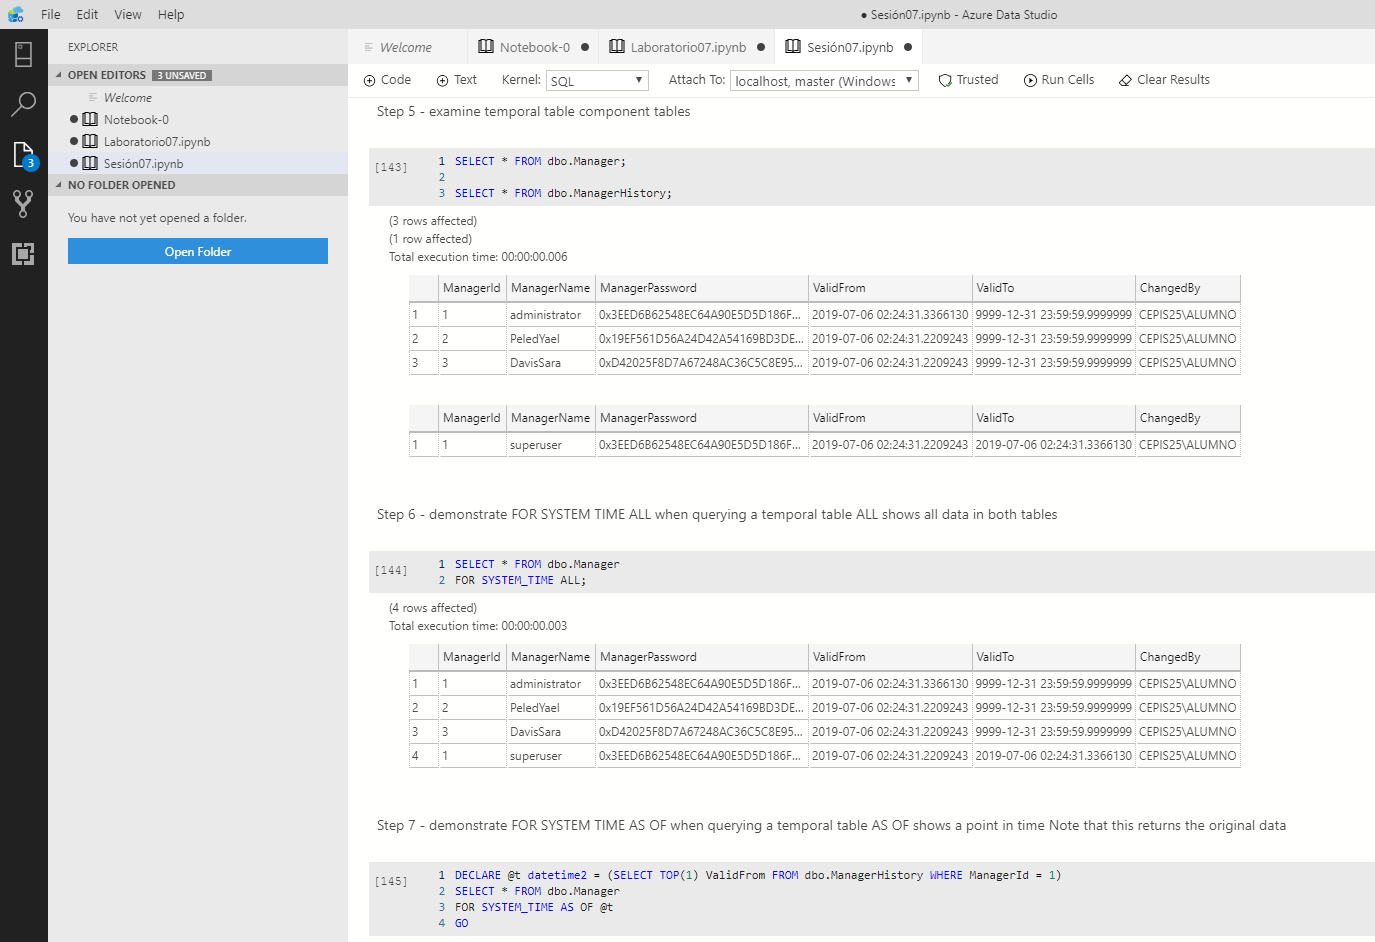
\includegraphics[width=15cm]{./Imagenes/1}
		\end{center}

\begin {itemize}
	\item Editor de código SQL con IntelliSense\\\\
	\subitem Azure Data Studio ofrece una experiencia moderna de codificación SQL centrada en el teclado que facilita sus tareas diarias con funciones integradas, como ventanas de pestañas múltiples, un editor de SQL enriquecido, IntelliSense, finalización de palabras clave, fragmentos de código, navegación de código y control de fuente integración (Git). Ejecute consultas SQL a pedido, vea y guarde los resultados como texto, JSON o Excel. Edite datos, organice sus conexiones de base de datos favoritas y explore los objetos de la base de datos en una experiencia familiar de búsqueda de objetos.
	\item Fragmentos de código de SQL inteligenter\\
	\subitem -Los fragmentos de código SQL generan la sintaxis SQL adecuada para crear bases de datos, tablas, vistas, procedimientos almacenados, usuarios, inicios de sesión, roles, etc., y para actualizar los objetos de base de datos existentes. Use fragmentos de código inteligente para crear rápidamente copias de su base de datos para fines de desarrollo o prueba, y para generar y ejecutar scripts CREAR e INSERTAR.\\\\
	\item Tableros personalizables de servidores y bases de datos\\
	\subitem -Cree ricos paneles personalizables para monitorear y solucionar rápidamente cuellos de botella de rendimiento en sus bases de datos. Para obtener información sobre los widgets de insight y los paneles de base de datos (y servidor), consulte Administrar servidores y bases de datos con widgets de insight .\\
	\item Gestión de la conexión (grupos de servidores)\\
	\subitem - Los grupos de servidores proporcionan una forma de organizar la información de conexión para los servidores y las bases de datos con las que trabaja. Para más detalles, consulte Grupos de servidores .\\\\
	\item Extensibilidad y autoría de extensión.\\
	\subitem - Mejore la experiencia de Azure Data Studio al ampliar la funcionalidad de la instalación básica. Azure Data Studio proporciona puntos de extensibilidad para las actividades de administración de datos, así como soporte para la creación de extensiones.\\
	
\end{itemize}






\section{PROCEDIMIENTO} 

\begin{itemize}
\subsection{Parte 1: Iniciando Docker:}
	\item Abrir el menu inicio y buscar la aplicación Docker for Windows.
                    \begin{figure}[H]
		\begin{center}
		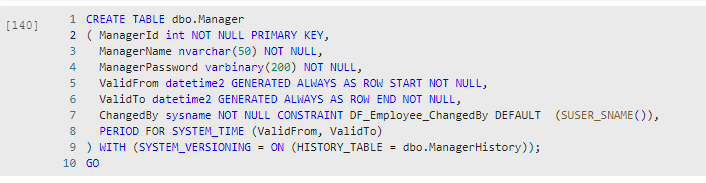
\includegraphics[width=7cm]{./Imagenes/s1}
		\end{center}
		\end{figure}
	\item Una vez iniciado se podrá visualizar el icono de Docker en el área de notificación.
   \begin{figure}[H]
		\begin{center}
		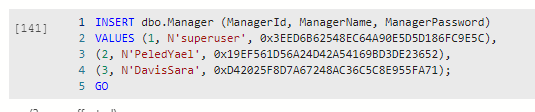
\includegraphics[width=7cm]{./Imagenes/s2}
		\end{center}
		\end{figure}
          \item Asimismo se podrá visualizar la ventana de bienvenida.
          \item Ingresar sus credenciales creadas en Docker Hub para iniciar sesión en el aplicativo..
   \begin{figure}[H]
		\begin{center}
		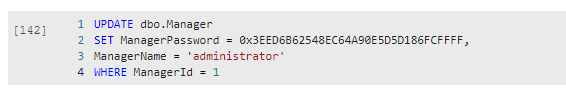
\includegraphics[width=7cm]{./Imagenes/s3}
		\end{center}
		\end{figure} 
          \item Ubicar la aplicación PowerShell, ejecutarla como Administrador. En la ventana de comandos de PowerShell escribir lo siguiente: "docker versión"
                       \begin{figure}[H]
		\begin{center}
		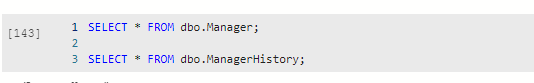
\includegraphics[width=7cm]{./Imagenes/s4}
		\end{center}
		\end{figure}   

                      \begin{figure}[H]
		\begin{center}
		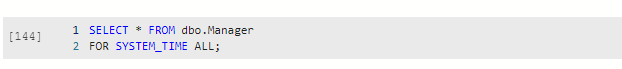
\includegraphics[width=7cm]{./Imagenes/s5}
		\end{center}
		\end{figure}   
         \item Verificar que el resultado sea el siguiente.
                     \begin{figure}[H]
		\begin{center}
		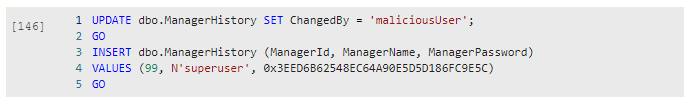
\includegraphics[width=7cm]{./Imagenes/s7}
		\end{center}
		\end{figure}   
\subsection{Parte 2: Creando un contenedor con Microsoft SQL Server para Linux}
	\item En la ventana de PowerShell, escribir el siguiente comando:"docker search mssql      
	\item El resultado deberá ser algo similar a lo siguiente.
                     \begin{figure}[H]
		\begin{center}
		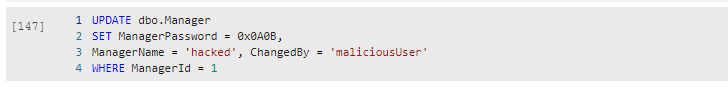
\includegraphics[width=15cm]{./Imagenes/s8}
		\end{center}
		\end{figure}   
	\item Ahora ejecutar el comando:"docker pull microsoft/mssql-server-linux"
	\item Lo cual descargará la imagen del contenedor de Microsoft SQL Server en un servidor Linux
                     \begin{figure}[H]
		\begin{center}
		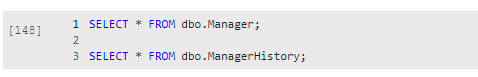
\includegraphics[width=15cm]{./Imagenes/s9}
		\end{center}
		\end{figure}   
          \item Proceder a verificar la imagen con el siguiente comando:" docker images"
	\item Lo cual deberá visualizar lo siguiente:
                     \begin{figure}[H]
		\begin{center}
		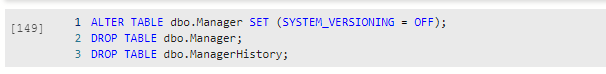
\includegraphics[width=15cm]{./Imagenes/s10}
		\end{center}
		\end{figure}   
	\item Seguidamente ejecutar el comando:
                      \begin{figure}[H]
		\begin{center}
		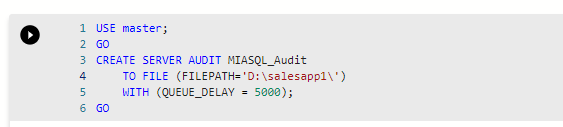
\includegraphics[width=15cm]{./Imagenes/s11}
		\end{center}
		\end{figure}   
	\item Como respuesta se visualizará un ID que corresponde al contenedor:
                     \begin{figure}[H]
		\begin{center}
		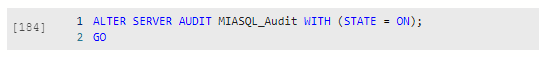
\includegraphics[width=15cm]{./Imagenes/s12}
		\end{center}
		\end{figure}   
           \item Verificar que el contenedor se este ejecutando correctamente mediante el comando:" docker ps"       
	\item Si se visualiza un cuadro de dialogo de permisos relacionados al firewall Windows, Aceptarlo para realizar la conexión.El resultado será similar al siguiente:
                     \begin{figure}[H]
		\begin{center}
		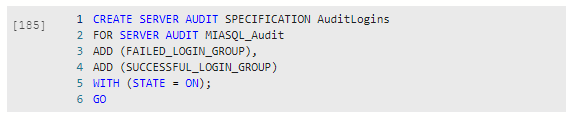
\includegraphics[width=15cm]{./Imagenes/s13}
		\end{center}
		\end{figure}   
	\item . Esperar unos segundos e iniciar la aplicación Microsoft SQL Server Management Studio, y conectar con los
siguientes datos:
                      \begin{figure}[H]
		\begin{center}
		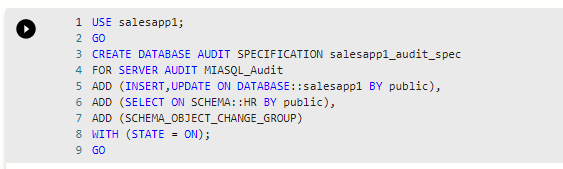
\includegraphics[width=15cm]{./Imagenes/s14}
		\end{center}
		\end{figure}   
	\item Iniciar una nueva consulta, escribir y ejecutar lo siguiente:
                     \begin{figure}[H]
		\begin{center}
		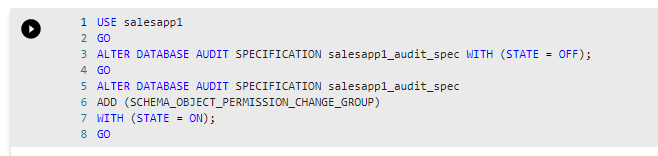
\includegraphics[width=15cm]{./Imagenes/s15}
		\end{center}
		\end{figure}   
          \item Deberá retornar algo similar a lo siguiente:
                     \begin{figure}[H]
		\begin{center}
		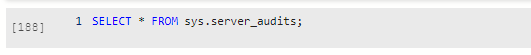
\includegraphics[width=15cm]{./Imagenes/s16}
		\end{center}
		\end{figure}   
	\item Cerrar la aplicación Microsoft SQL Server Management Studio.
	\item En PowerShell ejecutar el siguiente comando:" docker rm -f SQLLNX01"
                     \begin{figure}[H]
		\begin{center}
		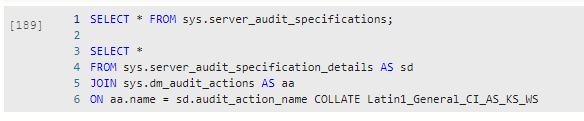
\includegraphics[width=15cm]{./Imagenes/s17}
		\end{center}
		\end{figure}   
	\item Verificar la eliminación del contenedor con ejecutando: docker ps
                    \begin{figure}[H]
		\begin{center}
		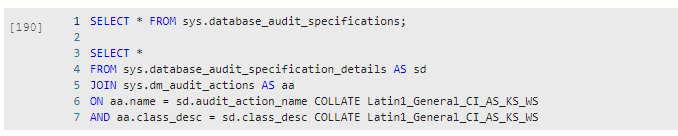
\includegraphics[width=15cm]{./Imagenes/s18}
		\end{center}
		\end{figure}   
\subsection{Parte 3: Adicionando persistencia}
	\item En PowerShell ejecutar el siguiente comando.
                     \begin{figure}[H]
		\begin{center}
		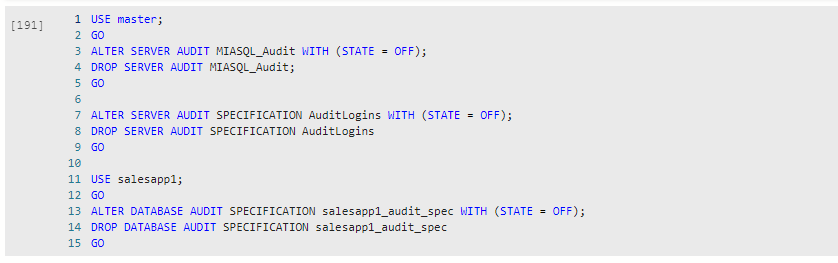
\includegraphics[width=15cm]{./Imagenes/s19}
		\end{center}
		\end{figure}   
          \item luego visualizara la siguiente ventana  ingresamos las credenciales.
                     \begin{figure}[H]
		\begin{center}
		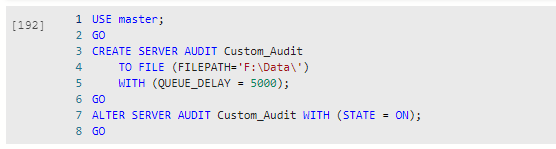
\includegraphics[width=15cm]{./Imagenes/s20}
		\end{center}
		\end{figure}   
	\item Como respuesta se visualizará un ID que corresponde al contenedor:
                     \begin{figure}[H]
		\begin{center}
		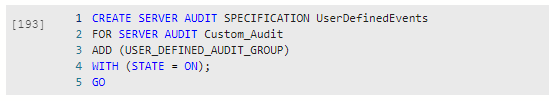
\includegraphics[width=15cm]{./Imagenes/s21}
		\end{center}
		\end{figure}   
	\item Verificar que el contenedor se este ejecutando correctamente mediante el comando:
                     \begin{figure}[H]
		\begin{center}
		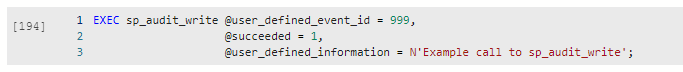
\includegraphics[width=15cm]{./Imagenes/s22}
		\end{center}
		\end{figure}   
           \item Esperar unos segundos e iniciar la aplicación Microsoft SQL Server Management Studio, y conectar con los siguientes datos:
                     \begin{figure}[H]
		\begin{center}
		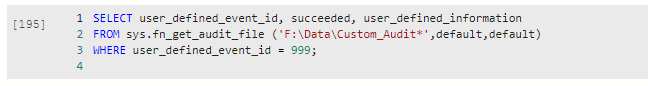
\includegraphics[width=15cm]{./Imagenes/s23}
		\end{center}
		\end{figure}   
	\item Generar una base de datos de prueba en la aplicación Microsoft SQL Server Management Studio, según la siguiente imagen mediante el siguiente script:
                     \begin{figure}[H]
		\begin{center}
		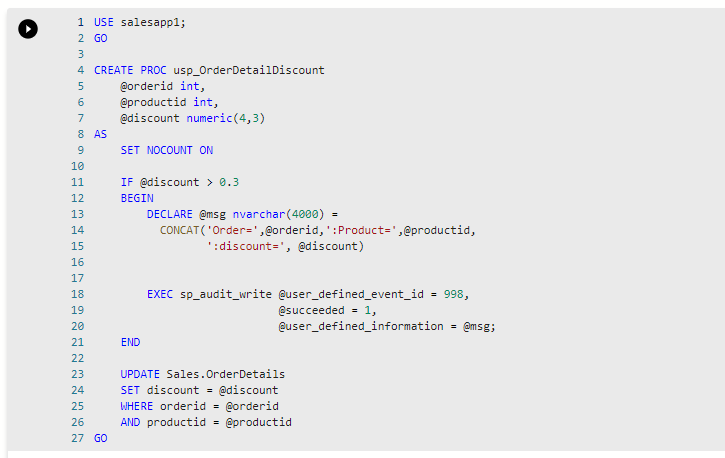
\includegraphics[width=15cm]{./Imagenes/s24}
		\end{center}
		\end{figure}   
           \item Verificar el contenido la carpeta DATALNX
                     \begin{figure}[H]
		\begin{center}
		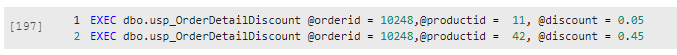
\includegraphics[width=15cm]{./Imagenes/s25}
		\end{center}
		\end{figure}   
           \item En PowerShell ejecutar el siguiente comando:"docker rm -f SQLLNX02"
                      \begin{figure}[H]
		\begin{center}
		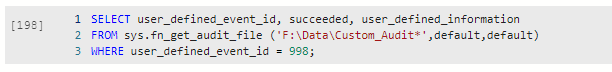
\includegraphics[width=15cm]{./Imagenes/s26}
		\end{center}
		\end{figure}   
	\item Verificar la eliminación del contenedor con ejecutando:"docker ps"
                    \begin{figure}[H]
		\begin{center}
		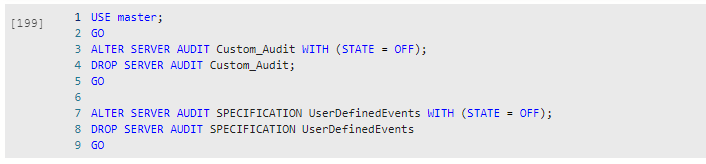
\includegraphics[width=15cm]{./Imagenes/s27}
		\end{center}
		\end{figure}   
\item antes se debe compartir o elnazar la carpeta  con Docker
                    \begin{figure}[H]
		\begin{center}
		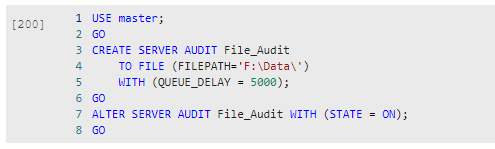
\includegraphics[width=15cm]{./Imagenes/s28}
		\end{center}
		\end{figure}   
\subsection{Parte 4: Creando un contenedor con Microsoft SQL Server para Windows}
	\item En el icono de Docker en el área de notificación, hacer click con el botón derecho y utilizar la opción Switch to Windows Containers. Esperar a que Docker se reinicie.
                      \begin{figure}[H]
		\begin{center}
		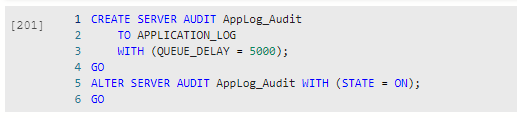
\includegraphics[width=10cm]{./Imagenes/s29}
		\end{center}
		\end{figure}   
                      \begin{figure}[H]
		\begin{center}
		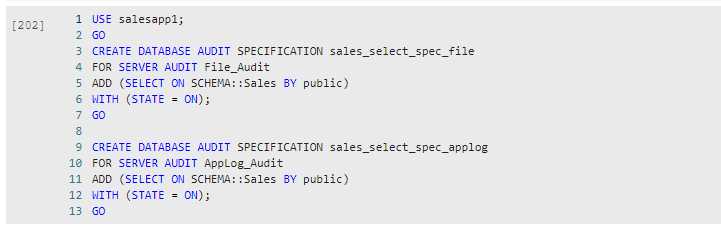
\includegraphics[width=10cm]{./Imagenes/s30}
		\end{center}
		\end{figure}   
	\item En la ventana de PowerShell, escribir el siguiente comando:"docker search mssql"           
                       \begin{figure}[H]
		\begin{center}
		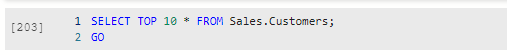
\includegraphics[width=15cm]{./Imagenes/s31}
		\end{center}
		\end{figure}   
          \item Ejecutar el siguiente comando; lo cual descargará la imagen del contenedor de Microsoft SQL Server en un servidor Linux.
		\begin{figure}[H]
		\begin{center}
		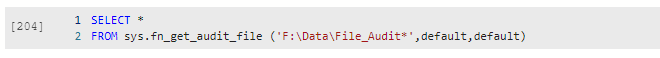
\includegraphics[width=15cm]{./Imagenes/s32}
		\end{center}
		\end{figure}  
         \item Proceder a verificar la imagen con el siguiente comando:
		\begin{figure}[H]
		\begin{center}
		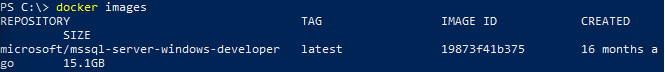
\includegraphics[width=15cm]{./Imagenes/c2}
		\end{center}
		\end{figure}  
          \item Seguidamente ejecutar el comando; como respuesta se visualizará un ID que corresponde al contenedor
		\begin{figure}[H]
		\begin{center}
		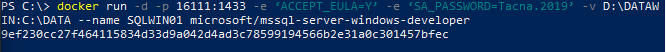
\includegraphics[width=15cm]{./Imagenes/c3}
		\end{center}
		\end{figure}  
          \item Repetir el paso 10 y verificar que el contenedor este ejecutándose
		\begin{figure}[H]
		\begin{center}
		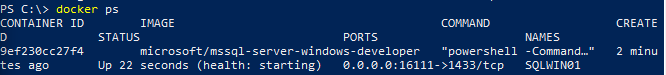
\includegraphics[width=15cm]{./Imagenes/c4}
		\end{center}
		\end{figure}  
          \item Repetir el paso 11 y conectar al servidor
		\begin{figure}[H]
		\begin{center}
		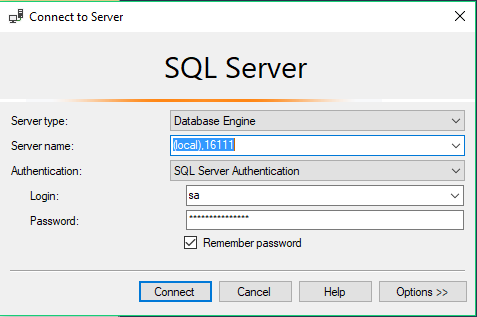
\includegraphics[width=15cm]{./Imagenes/c5}
		\end{center}
		\end{figure}  
         \item Iniciar una nueva consulta, escribir y ejecutar lo siguiente:
		\begin{figure}[H]
		\begin{center}
		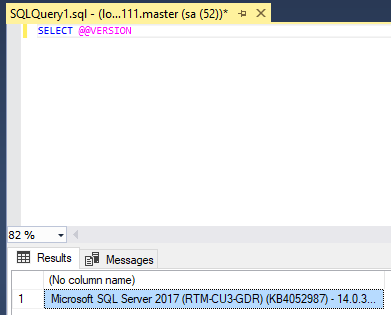
\includegraphics[width=10cm]{./Imagenes/c6}
		\end{center}
		\end{figure}  
          \item Generar una base de datos de prueba en la aplicación Microsoft SQL Server Management Studio
		\begin{figure}[H]
		\begin{center}
		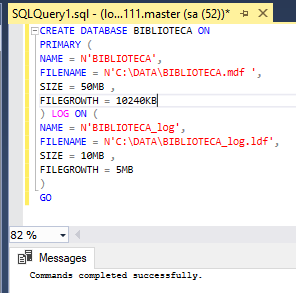
\includegraphics[width=10cm]{./Imagenes/c7}
		\end{center}
		\end{figure}  
          \item Verificar el contenido de la carpeta DATAWIN
		\begin{figure}[H]
		\begin{center}
		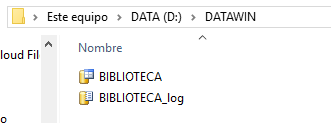
\includegraphics[width=12cm]{./Imagenes/c8}
		\end{center}
		\end{figure}  
         \item En PowerShell ejecutar el siguiente comando y verificar la eliminación del contenedor con ejecutando
		\begin{figure}[H]
		\begin{center}
		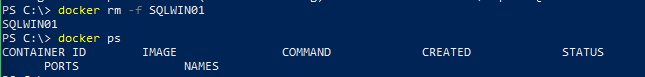
\includegraphics[width=15cm]{./Imagenes/c9}
		\end{center}
		\end{figure}  
          \item Cerrar la aplicación Microsoft SQL Server Management Studio.
       
\end{itemize}
		
\section{ANALISIS E INTERPRETACION DE RESULTADOS} 


\subsection{Parte 1: Actividades Encargadas}
	\begin{itemize}
		\item ¿Con qué comando(s) exportaría la imagen de Docker de Microsoft SQL Server a otra PC o servidor?
                      \begin{figure}[H]
		\begin{center}
		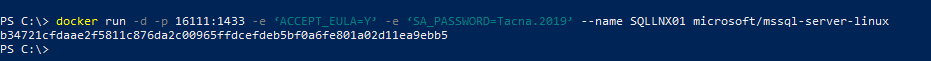
\includegraphics[width=15cm]{./Imagenes/6}
		\end{center}
		\end{figure} 
		\item ¿Con qué comando(s) podría generar dos volúmenes para un contenedor para distribuir en un volumen el Archivo de Datos (.mdf) y en otro el Archivo Log (.ldf)? 
                     \begin{figure}[H]
		\begin{center}
		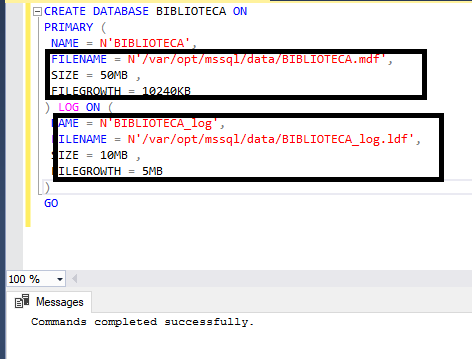
\includegraphics[width=7cm]{./Imagenes/18}
		\end{center}
		\end{figure} 
		\item Genere un nuevo contenedor y cree la base de datos con las siguientes características.
                      \begin{figure}[H]
		\begin{center}
		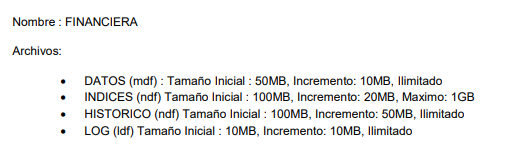
\includegraphics[width=7cm]{./Imagenes/30}
		\end{center}
		\end{figure} 
		\item  ¿Cuál sería el script SQL que generaría esta base de datos?
\begin{figure}[H]
		\begin{center}
		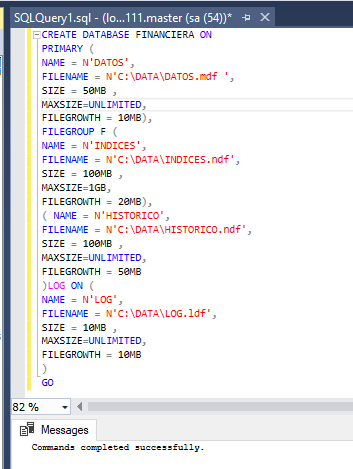
\includegraphics[width=10cm]{./Imagenes/t4}
		\end{center}
		\end{figure}
	\end{itemize}




\section{CONCLUSIONES}
\begin{itemize}
	\item En conclusión hemos observado y experimentado con docker, y nos resulta que es muy util al momento de instalar multiples bases de datos y que no existe la necesidad de armar o instalar múltipler ordenadores físicos o virtuales.
	
	\item Es por eso que resulta factible en muchos aspectos como migrar de version, tener varias bases de datos disponibles o además que existieran y comparen diferentes versiones de bases de datos a la vez
\end{itemize}

\newpage

\section{REFERENCIAS} 

\begin{itemize}
	\item [[ 1]] Hat, R. (2017). ¿Qué es Docker?. Recuperado de https://www.redhat.com/es/topics/containers/what-is-docker
	\item  [[ 2]] Why Docker? | Docker. (2017). Recuperado de https://www.docker.com/why-docker
 	\item   [[ 3]] Araujo, J. (2017). ¿Qué es Docker? ¿Que son los contenedores? y ¿Por que no usar VMs?. Recuperado de https://platzi.com/contributions/guia-del-curso-de-docker/
	\item  [[ 4]]  Oterino, A. (2015). ¿Qué es Docker? ¿Para qué se utiliza? Explicado de forma sencilla. Recuperado de https://www.javiergarzas.com/2015/07/que-es-docker-sencillo.html
\end{itemize}




\end{document}
